% -----------------------------------------------------------------
% Desenvolvido por Filipe Fernandes para o LIPES (Laboratório de Inovação, Pesquisa e Engenharia de Software)
% filipe.fernandes@ifsudestemg.edu.br
% ----------------------------------------------------------------
% Adaptado de Template Latex - Apresentação - UFMG
% https://www.overleaf.com/latex/templates/template-latex-apresentacao-ufmg/ygvvbrrsqgkv
% -----------------------------------------------------------------
% Licença Creative Commons CC BY 4.0
% -----------------------------------------------------------------
% PARA CORRER pdflatex -shell-escape main.tex
\documentclass[aspectratio=169,english]{beamer}

% a opção hideSubsectionTitle esconde o título das subseções
\usepackage{templateLIPES}      % o arquivo templateLIPES.sty possui todo o estilo de formatação
\usepackage[spanish]{babel}     % mude o idioma, caso necessite
\usepackage[alf, abnt-emphasize=bf, abnt-etal-text=it]{abntex2cite}

\setbeamertemplate{bibliography item}{}
\renewcommand{\theenumiv}{}

\begin{document}

\titulo{Incorporación de técnicas de muestreo mediante histogramas multidimensionales al código de
simulación de fuentes de Monte Carlo KDSource}
% \subtitulo{Subtítulo}       % caso não haja, comente

\autor{Lucas Ezequiel Ovando}
\orientador{Dr. Ariel Marquez}        % caso não haja, comente
\coorientador{Ing. Zoe Prieto}      % caso não haja, comente

\curso{Ingenieria Nuclear}

\local{San Carlos de Bariloche, Rio Negro, Argentina}
\dia{16}
\mes{febrero}
\ano{2025}

% NÃO REMOVA!
\begin{frame}[plain]
    
    \begin{tikzpicture}[overlay,remember picture]
        \node[left=-0.15cm] at (current page.0){
            
\includegraphics[scale=0.145]{imagens/capaLIPES}
        };
    \end{tikzpicture}

    \titlepage
    
\end{frame}

\section[Resumen]{}

\begin{frame}[allowframebreaks]
    \frametitle{Resumen}
    \tableofcontents
\end{frame}

% CONTEÚDO -----------------------------------------------------------------

\section{Introdución}
\begin{frame}{Introdución}
    En este trabajo se planea incorporar una:
    \begin{itemize}
        \item tecnica de muestreo...
        \item ... mediante histogramas multidimensionales...
        \item ... al codigo de simulacion de fuentes Monte Carlo KDSource
    \end{itemize}
\end{frame}

\begin{frame}{Introdución: Tecnica de muestreo}
    \begin{figure}
        \centering
        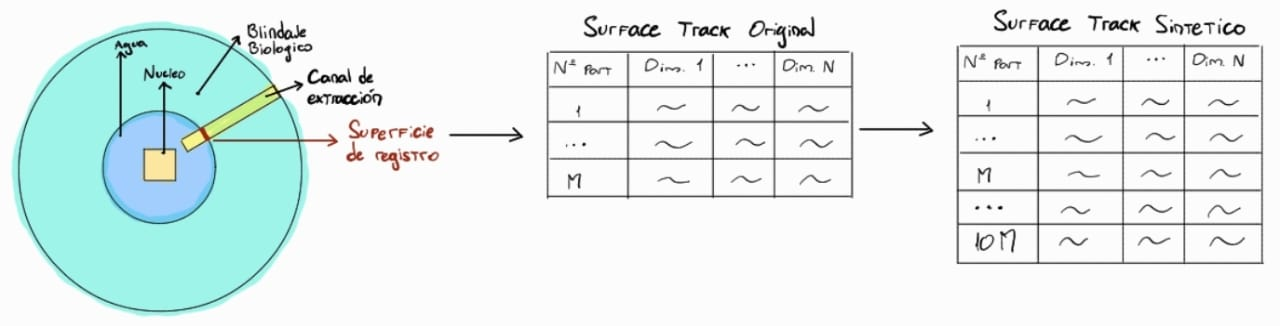
\includegraphics[width=1\linewidth]{imagens/esquema1.jpeg}
        % \caption{1º seminário do LIPES em 27/01/2025}
        \label{fig:esquema1}
    \end{figure}

    Idea: a partir de una simulacion Monte Carlo donde se registran las particulas que atraviesan una superficie
    de registro se obtiene un surface track original. Luego se genera un surface track sintetico de mayor tamaño 
    para continuar la simulacion desde esa superficie en adelante.
\end{frame}

\begin{frame}{Introdución: Histogramas multidimensionales}
    \begin{figure}
        \centering
        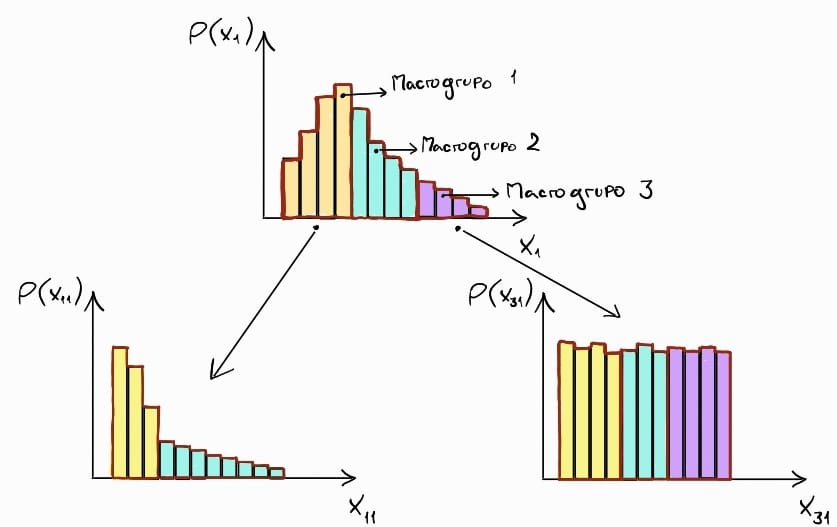
\includegraphics[width=0.35\linewidth]{imagens/esquema2.jpeg}
        % \caption{1º seminário do LIPES em 27/01/2025}
        \label{fig:esquema2}
    \end{figure}

    Idea: realizar un histograma de la primer variable para luego subdividir la variable en macro grupos. Luego se 
    realiza subsiguientes histogramas de la siguiente variable para cada macro grupo. Se repite el proceso hasta formar
     un arbol de histogramas multidimensionales.

    Esto se realiza para poder obtener aproximaciones de la distribucion de probabilidad de las variables de interes mientras 
    se conserva la correlacion entre las variables.
\end{frame}

\begin{frame}{Introdución: Codigo de simulación de fuentes Monte Carlo KDSource}
    \begin{figure}
        \centering
        
\includegraphics[width=0.35\linewidth]{imagens/esquema3.png}
        % \caption{1º seminário do LIPES em 27/01/2025}
        \label{fig:esquema3}
    \end{figure}

    Idea: KDSource es un codigo de simulacion de fuentes de Monte Carlo que se formulo en la tesis de maestria de 
    Inti Osiris Abbate para el codigo de fuente libre OpenMC. 
    
    El mismo actualmente permite simular fuentes de neutrones y fotones 
    a traves del metodo KDE. Se planea aprovechar la plataforma de KDSource para incorporar las tecnicas de muestreo
    mediante histogramas multidimensionales.
\end{frame}

\section{Motivación}
\begin{frame}{Motivación}
    % \begin{figure}
    %     \centering
    %     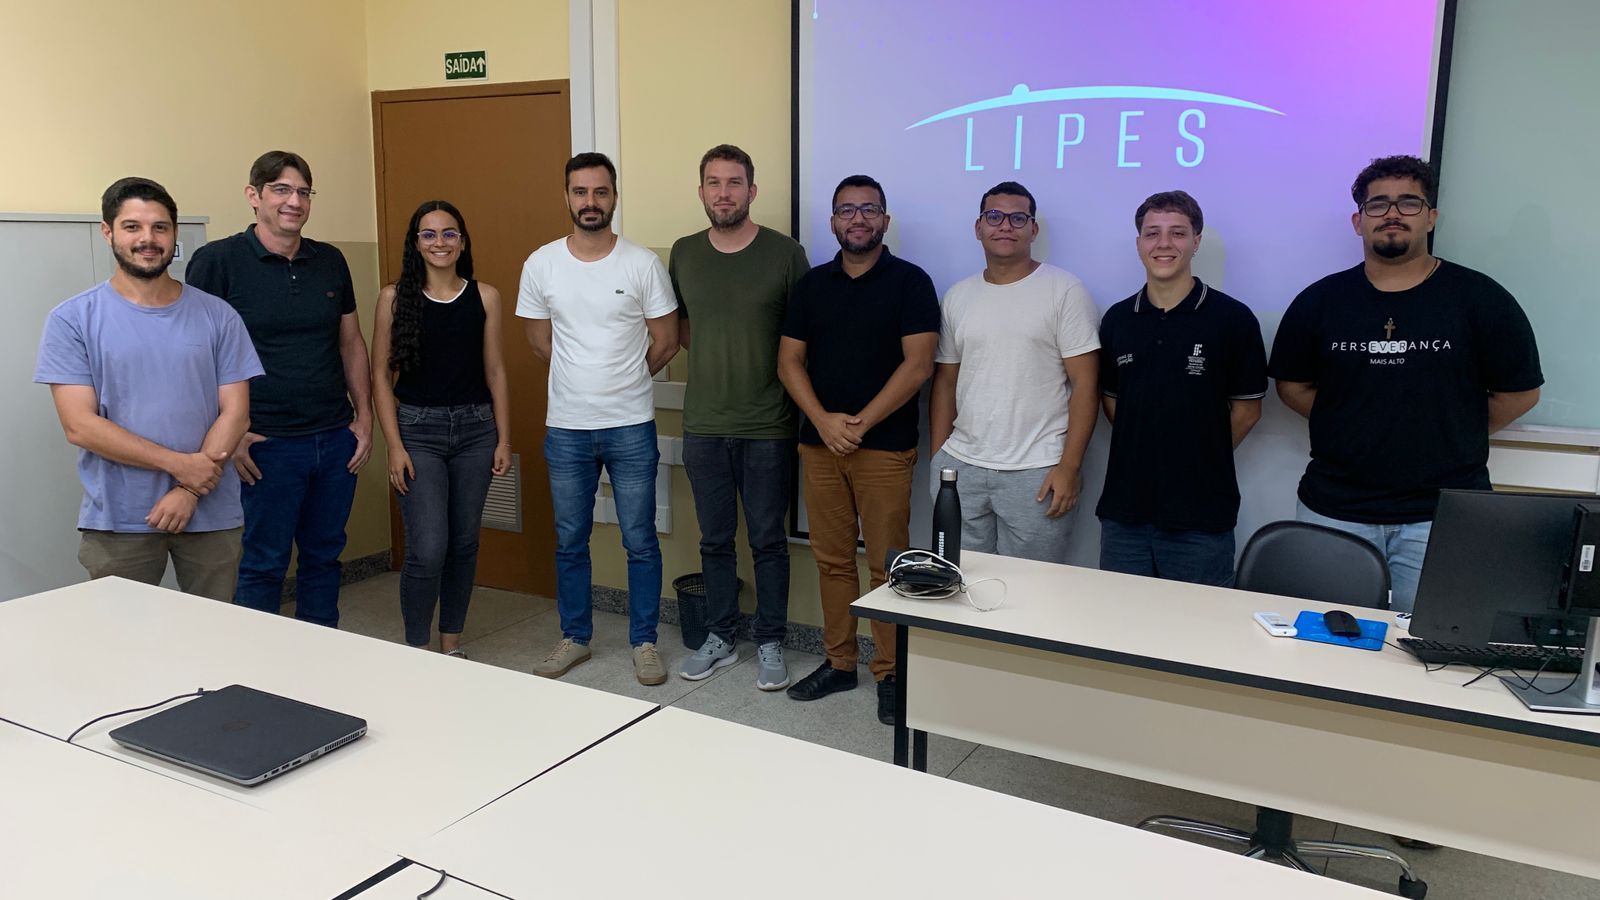
\includegraphics[width=0.6\linewidth]{imagens/1_seminario_LIPES.jpeg}
    %     % \caption{1º seminário do LIPES em 27/01/2025}
    %     \label{fig:1semlipes}
    % \end{figure}
    En problemas de transporte de radiación aplicados a calculo de blindajes y extraccion de 
    haces de neutrones se presenta la necesidad de obtener el flujo de radiacion a grandes 
    distancias del nucleo del reactor. Ademas, el calculo de blindajes trae el problema intrinseco 
    de querer obtener el flujo de radiacion en puntos donde se espera que haya bajo flujo.
    La forma de reducir el tiempo de calculo en estos problemas es la incorporacion de tecnicas de 
    reducción de varianza. Con estas es posible obtener tiempos razonables de simulación.
    
    Con este objetivo se plantea la incorporacion de tecnicas de muestreo mediante histogramas 
    multidimensionales al codigo de simulacion de fuentes de Monte Carlo KDSource.
\end{frame}

\section{Trabajo en curso}
\begin{frame}{Trabajo en curso}
    Avances hasta el momento:
    \begin{itemize}
        \item Interiorización del problema y de las tecnicas a incorporar
        \item Creación de un metodo para la aproximación de la distribucion de probabilidad de las variables de interes a traves de histogramas multidimensionales en python. Por el momento requiere del usuario para la seleccion de parametros. Hasta el momento por fuera del codigo de KDSource. 
        \item Creación de un metodo para la generación de surface tracks sinteticos a partir de los histogramas multidimensionales en python. Hasta el momento falta traducirlo a C para poder incorporarlo al codigo de KDSource.
        \item Resultados parciales en un ejemplo de simulacion similar a un haz de extraccion de neutrones.
        \item Todo el trabajo se ha realizado para neutrones, excluyendo los fotones.
    \end{itemize}
    % \begin{figure}
    %     \centering
    %     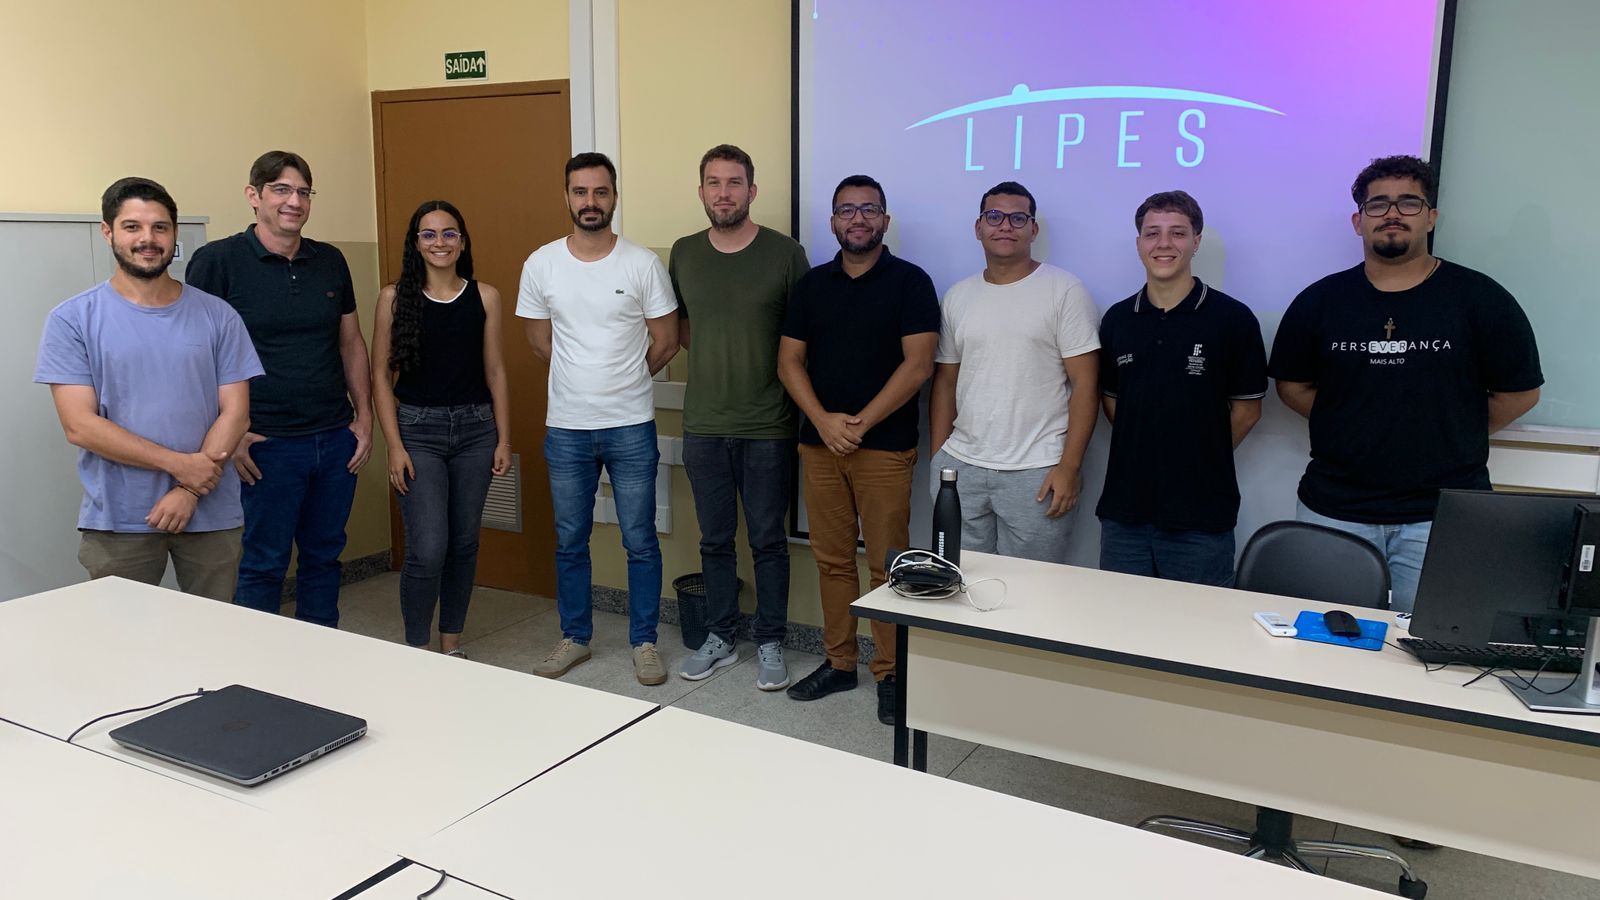
\includegraphics[width=0.6\linewidth]{imagens/1_seminario_LIPES.jpeg}
    %     % \caption{1º seminário do LIPES em 27/01/2025}
    %     \label{fig:1semlipes}
    % \end{figure}

\end{frame}

\begin{frame}{Trabajo en curso: Histogramas multidimensionales}
    Hasta aca llego por hoy. La idea es comentar en esta subseccion la forma en la que, a traves de inputs del usuario, se generan los histogramas macro y micro. Ademas de comentar que se pueden incorporar bordes de los macrogrupos de forma manual
    para fortalecer la correlacion entre las variables. Por ejemplo los limites geometricos del canal de extracción. 
    Tambien busco comentar la estructura tipo arbol que se forma con los histogramas multidimensionales y dar una idea de los tamaños tipicos con un ejemplo.
    Ademas comentar las ventajas y desventajas de incorporar diferentes cantidades de macro y microgrupos. (macro ancho: mayor estadistica. macro fino: mayor correlacion entre variables. micro ancho: se pierde detale. micro fino: se copia el ruido estadistico)

    ------------

    En la siguiente diapositiva explicar el metodo de sampleo de las variables a partir de los histogramas multidimensionales. Aca incorporar los numeros pseudoaleatorios y la utilizacion de las funciones de frecuencia acumulada.

    % \begin{figure}
    %     \centering
    %     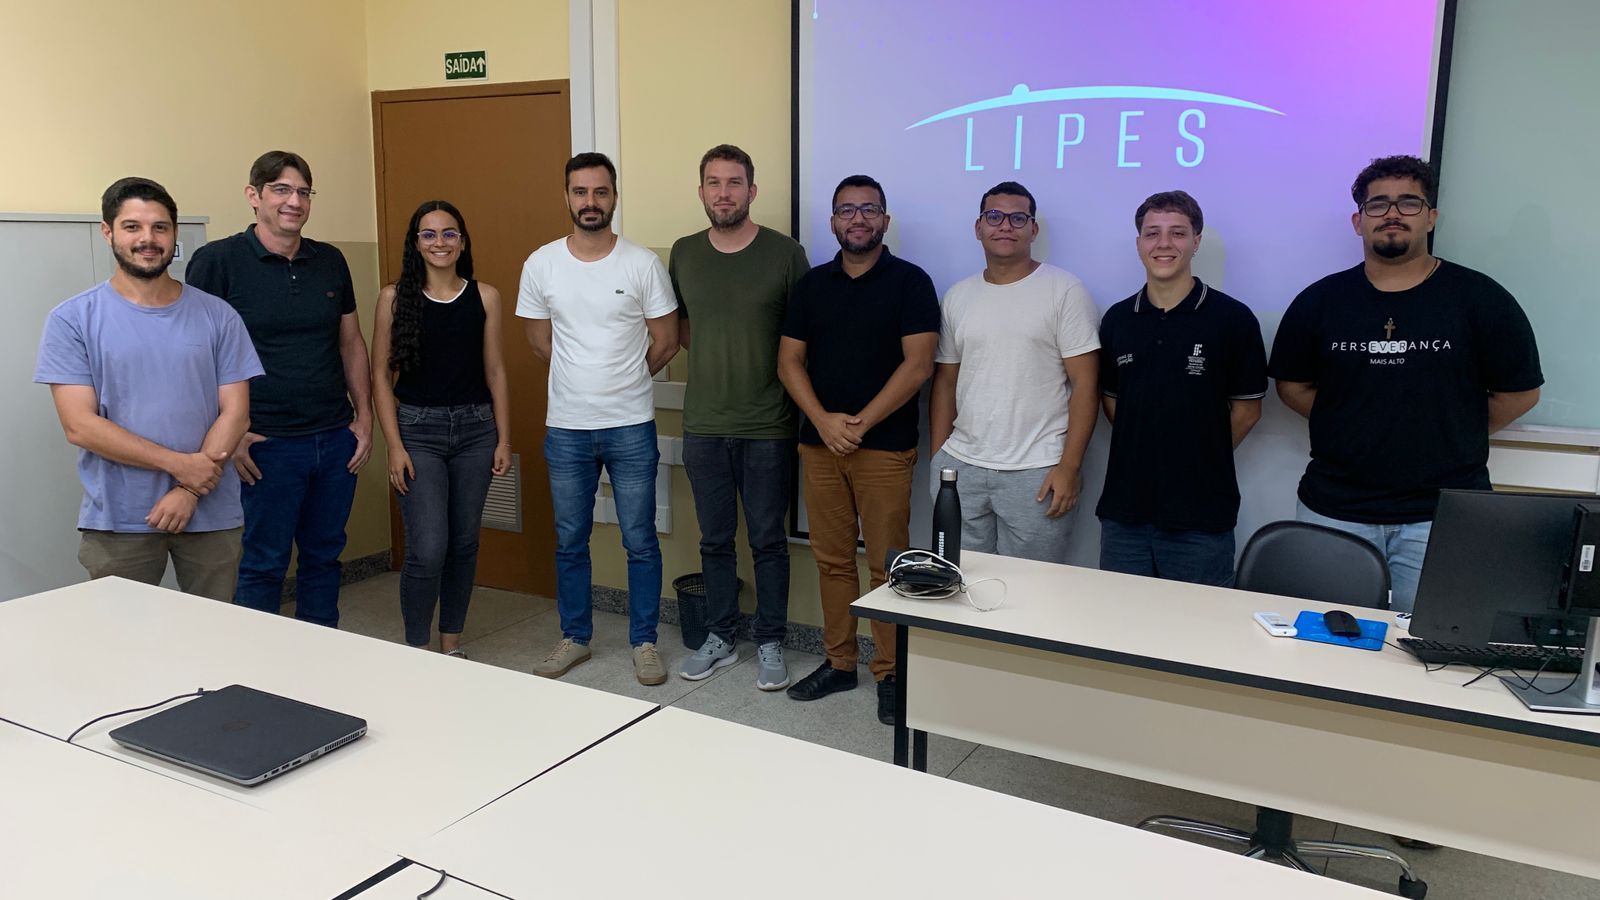
\includegraphics[width=0.6\linewidth]{imagens/1_seminario_LIPES.jpeg}
    %     % \caption{1º seminário do LIPES em 27/01/2025}
    %     \label{fig:1semlipes}
    % \end{figure}

\end{frame}

\begin{frame}{Trabajo en curso: Histogramas multidimensionales}
    Por ultimo comentar el ejemplo de aplicacion que venimos trabajando y los resultados parciales que hemos obtenido. Entre ellos comentar diferencias entre incorporar o no los limites manuales de los macrogrupos (geometricos y en letargia). Ademas comentar diferencias entre diferente cantidad de micro y macrogrupos. Y tambien entre mayor o menor cantidad de particulas registradas.
    Ademas comentar del tubo de vacio y caracteristicas delticas de la fuente que estamos utilizando (delta en mu y en letargia).
    Ademas comentar que miramos el flujo a traves de la dimension de propagacion (total, agua y vacio) y que se observa el espectro al final del tubo (total, agua y vacio).

    ------------ 
    
    Por no tan ultimo comentar trabajo a futuro:
    - Seleccion de parametros automatica con menor intervencion del usuario.
    - Traducir el sampleo de python a C.
    - Aplicacion en el conducto N5 del RA6 para la simulacion del CHOPPPER.

    % \begin{figure}
    %     \centering
    %     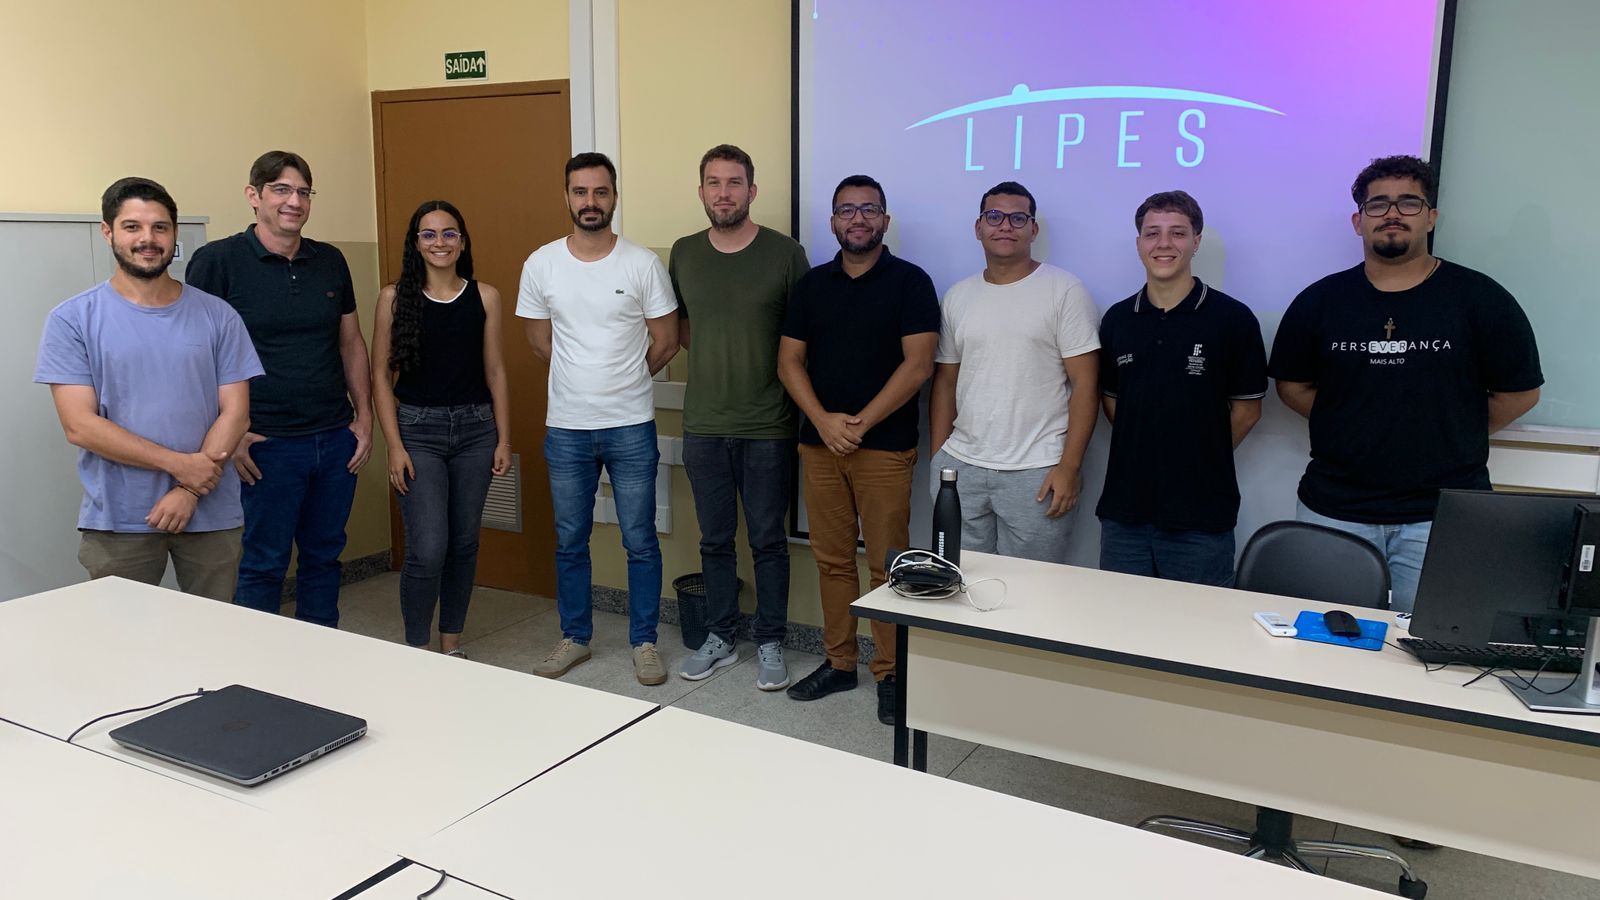
\includegraphics[width=0.6\linewidth]{imagens/1_seminario_LIPES.jpeg}
    %     % \caption{1º seminário do LIPES em 27/01/2025}
    %     \label{fig:1semlipes}
    % \end{figure}

\end{frame}

% \section{Código}
% \begin{frame}[fragile]{Código}
% \begin{minted}{python}
% from qiskit import QuantumRegister, QuantumCircuit
% from numpy import pi

% qreg_q = QuantumRegister(2, 'q')
% circuit = QuantumCircuit(qreg_q)

% circuit.h(qreg_q[0])
% circuit.cx(qreg_q[0], qreg_q[1])
% \end{minted}
% \end{frame}

% \section{Citação}
% \begin{frame}{Citação}
%     \begin{itemize}
%         \item De acordo com \citeonline{fernandes2017} ...
%         \item ... lorem ipsum \cite{fernandes2023}.
%     \end{itemize}
% \end{frame}

% FIM DO CONTEÚDO -----------------------------------------------------------------

% NÃO REMOVA!
\section{Referências}
\begin{frame}[allowframebreaks]
    \addtocounter{framenumber}{-1}
    \frametitle{Referências}
    \scriptsize
    % \bibliographystyle{abntex2-alf-en}  % mude para qualquer arquivo .bst
    \bibliography{referencias}
\end{frame}     
\end{document}